\documentclass[tikz,border=10pt]{standalone}
\usepackage{amsmath}
\usepackage{newtxtext,newtxmath}
\usetikzlibrary{arrows.meta,positioning,fit,backgrounds,calc,
  decorations.pathmorphing,shapes.misc}

% ---- palette --------------------------------------------------------------
\definecolor{ink}{HTML}{1B2A38}
\definecolor{acc}{HTML}{0A8F9E}
\definecolor{accfill}{HTML}{E7F4F5}
\definecolor{panel}{HTML}{F5F7F9}
\definecolor{line}{HTML}{C7D2DA}
\definecolor{cdelta}{HTML}{3B5BD0}\definecolor{ctheta}{HTML}{6741C9}
\definecolor{calpha}{HTML}{0F9D76}\definecolor{cbeta}{HTML}{D18A00}
\definecolor{cgamma}{HTML}{D1541F}\definecolor{tgt}{HTML}{8795A1}

\begin{document}
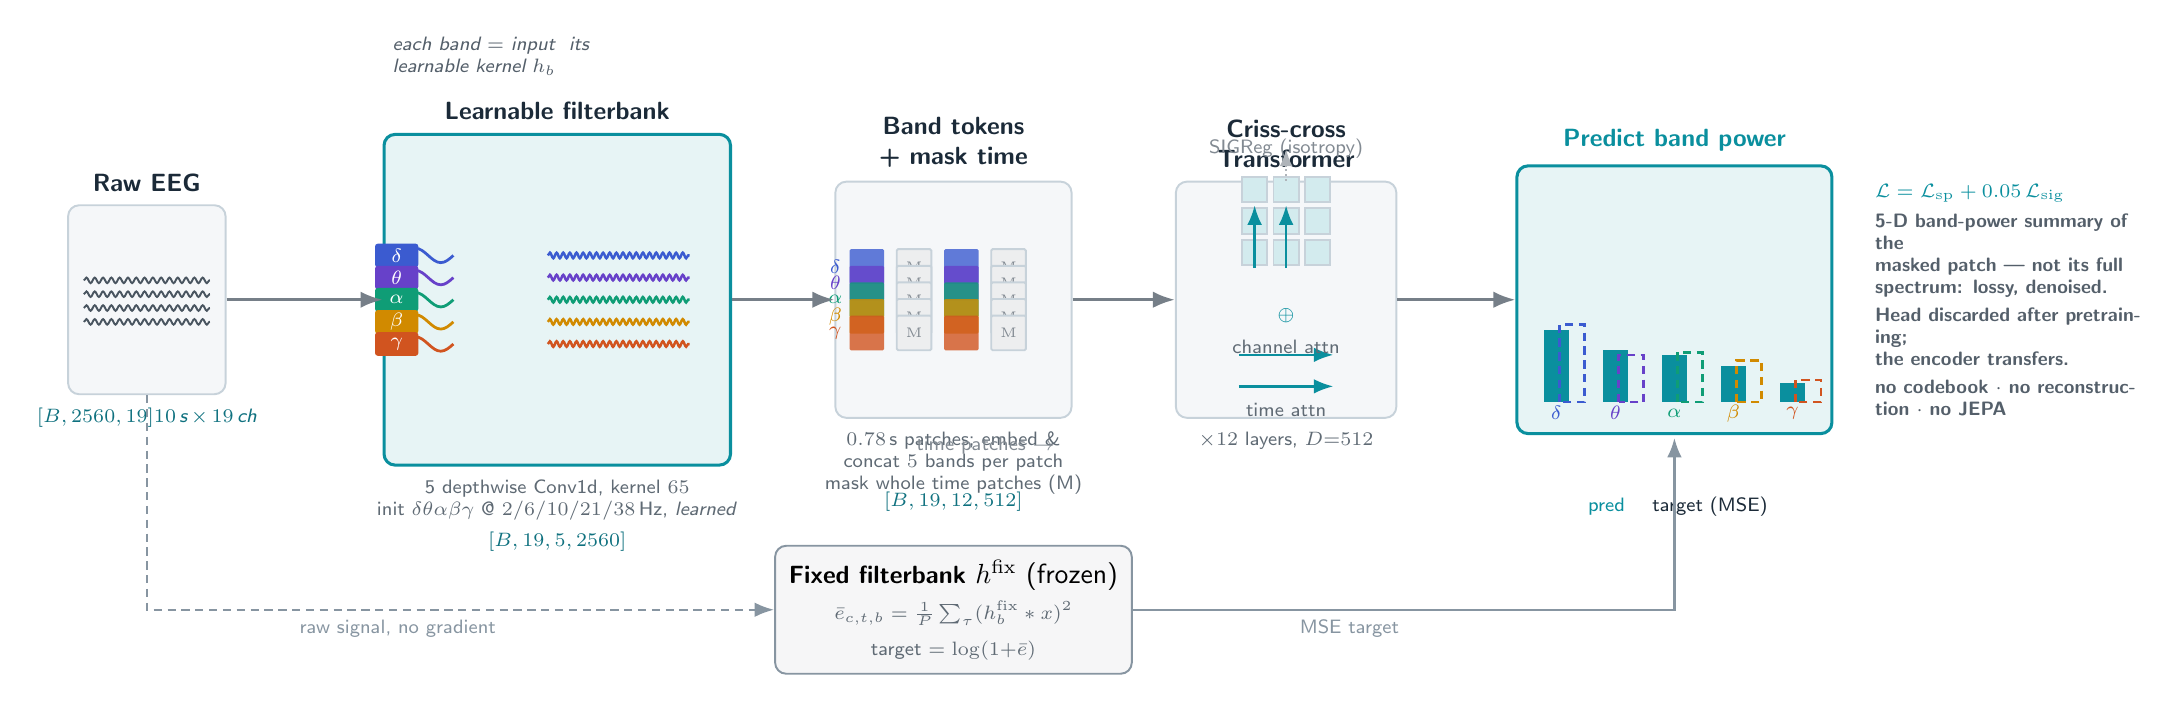
\begin{tikzpicture}[font=\sffamily,>=Latex,line width=.7pt,
  stage/.style={draw=line,rounded corners=4pt,fill=panel,inner sep=5pt,align=center},
  accstage/.style={draw=acc,line width=1.1pt,rounded corners=4pt,fill=accfill,
    inner sep=5pt,align=center},
  lbl/.style={font=\sffamily\small\bfseries,text=ink},
  sub/.style={font=\sffamily\scriptsize,text=ink!70,align=center},
  dim/.style={font=\sffamily\scriptsize\itshape,text=acc!70!ink},
  ann/.style={font=\sffamily\scriptsize,text=ink!75,align=left},
  flow/.style={->,draw=ink!60,line width=1.1pt},
  band/.style={font=\sffamily\scriptsize\bfseries,text=white,inner sep=0pt}]

% ============================================================= 1. INPUT
\node[stage,minimum width=20mm,minimum height=24mm] (in) {};
\foreach \y/\f in {7/9, 2/13, -3/6, -8/17}{
  \draw[ink!80,line width=.7pt,decorate,
    decoration={snake,amplitude=1pt,segment length=3pt}]
    ($(in.center)+(-8mm,\y pt)$) -- ++(16mm,0);}
\node[lbl,above=1pt of in] {Raw EEG};
\node[dim,below=1pt of in] {$[B,2560,19]$\\ $10$\,s\,$\times$\,$19$\,ch};

% ============================================================= 2. FILTERBANK (conv)
\coordinate (fbanchor) at ($(in.east)+(20mm,0)$);
\node[accstage,minimum width=44mm,minimum height=42mm] (fb) at ($(fbanchor)+(22mm,0)$) {};
% 5 learnable kernels, each convolved with the input -> a band
\foreach \c/\n/\yy in {cdelta/$\delta$/16, ctheta/$\theta$/8, calpha/$\alpha$/0,
                       cbeta/$\beta$/-8, cgamma/$\gamma$/-16}{
  % kernel icon (small sinusoid, drawn with built-in sin/cos path ops)
  \draw[\c,line width=1pt] ($(fb.west)+(2.6mm,\yy pt)$)
     sin ++(1.6mm,2.6pt) cos ++(1.6mm,-2.6pt) sin ++(1.6mm,-2.6pt) cos ++(1.6mm,2.6pt);
  \node[band,fill=\c,rounded corners=1pt,minimum width=5.5mm,minimum height=3mm]
     at ($(fb.west)+(1.8mm,\yy pt)$) {\n};
  % convolution symbol
  \node[font=\small,text=ink] at ($(fb.west)+(17mm,\yy pt)$) {$\circledast$};
  % resulting band trace
  \draw[\c,line width=.9pt,decorate,decoration={snake,amplitude=1pt,segment length=2.4pt}]
     ($(fb.west)+(21mm,\yy pt)$) -- ++(18mm,0);
}
\node[lbl,above=1pt of fb,align=center] {Learnable filterbank};
\node[sub,below=1pt of fb] {5 depthwise Conv1d, kernel $65$\\
  init $\delta\theta\alpha\beta\gamma$ @ $2/6/10/21/38$\,Hz, \emph{learned}};
\node[dim,below=7mm of fb] {$[B,19,5,2560]$};
\node[ann,above=6mm of fb.north west,anchor=south west,text width=30mm]
  {\itshape each band $=$ input $\circledast$ its\\ learnable kernel $h_b$};

% ============================================================= 3. TOKENS + MASK
\node[stage,minimum width=30mm,minimum height=30mm,right=13mm of fb] (tok) {};
\foreach \gl/\c/\yy in {\delta/cdelta/12, \theta/ctheta/6, \alpha/calpha/0,
                        \beta/cbeta/-6, \gamma/cgamma/-12}{
  \foreach \t/\xx in {0/-11,1/-5,2/1,3/7}{
     \pgfmathsetmacro\m{(\t==1 || \t==3)?1:0}
     \ifnum\m=1
        \node[draw=line,fill=ink!8,minimum size=4.4mm,inner sep=0,rounded corners=.5pt,
          font=\tiny,text=ink!55] at ($(tok.center)+(\xx mm,\yy pt)$) {M};
     \else
        \node[fill=\c,fill opacity=.8,minimum size=4.4mm,inner sep=0,rounded corners=.5pt]
          at ($(tok.center)+(\xx mm,\yy pt)$){};
     \fi}
  \node[font=\scriptsize] at ($(tok.center)+(-15mm,\yy pt)$) {\color{\c}$\gl$};
}
\node[lbl,above=1pt of tok,align=center] {Band tokens\\+ mask time};
\node[sub,below=1pt of tok] {$0.78$\,s patches; embed \&\\ concat $5$ bands per patch\\ mask whole time patches (M)};
\node[dim,below=8mm of tok] {$[B,19,12,512]$};
\node[sub,below right=1mm and -6mm of tok.south]{\color{ink!55}time patches $\rightarrow$};

% ============================================================= 4. CRISS-CROSS ENCODER
\node[stage,minimum width=28mm,minimum height=30mm,right=13mm of tok] (enc) {};
% mini token grid
\foreach \r in {0,1,2}\foreach \cix in {0,1,2}{
  \node[draw=line,fill=acc!18,minimum size=3.2mm,inner sep=0]
    at ($(enc.center)+({(\cix-1)*4mm},{(\r-0)*4mm+6mm})$){};}
% channel-attention arrows (vertical)
\draw[->,acc,line width=.9pt] ($(enc.center)+(-4mm,4mm)$) -- ++(0,8mm);
\draw[->,acc,line width=.9pt] ($(enc.center)+(0,4mm)$) -- ++(0,8mm);
\node[sub,text=acc] at ($(enc.center)+(0mm,-2mm)$) {$\oplus$};
% time-attention arrows (horizontal)
\draw[->,acc,line width=.9pt] ($(enc.center)+(-6mm,-7mm)$) -- ++(12mm,0);
\draw[->,acc,line width=.9pt] ($(enc.center)+(-6mm,-11mm)$) -- ++(12mm,0);
\node[sub] at ($(enc.center)+(0,-6mm)$) {\color{ink!70}channel attn};
\node[sub] at ($(enc.center)+(0,-14mm)$) {\color{ink!70}time attn};
\node[lbl,above=1pt of enc,align=center] {Criss-cross\\Transformer};
\node[sub,below=1pt of enc] {$\times 12$ layers, $D{=}512$};

% ============================================================= 5. BAND-POWER HEAD (star)
\node[accstage,minimum width=40mm,minimum height=34mm,right=15mm of enc] (bp) {};
% bars: pred (solid) vs target (dashed)
\def\base{-13mm}
\foreach \c/\xx/\hp/\ht in {cdelta/-15/26/28, ctheta/-7.5/19/17, calpha/0/17/18,
                            cbeta/7.5/13/15, cgamma/15/7/8}{
  \fill[acc] ($(bp.center)+(\xx mm-1.6mm,\base)$) rectangle ++(3.2mm,\hp pt);
  \draw[\c,line width=1pt,densely dashed] ($(bp.center)+(\xx mm+0.4mm,\base)$)
     rectangle ++(3.2mm,\ht pt);
}
\node[sub] at ($(bp.center)+(-15mm,\base)+(0,-4pt)$){\color{cdelta}$\delta$};
\node[sub] at ($(bp.center)+(-7.5mm,\base)+(0,-4pt)$){\color{ctheta}$\theta$};
\node[sub] at ($(bp.center)+(0,\base)+(0,-4pt)$){\color{calpha}$\alpha$};
\node[sub] at ($(bp.center)+(7.5mm,\base)+(0,-4pt)$){\color{cbeta}$\beta$};
\node[sub] at ($(bp.center)+(15mm,\base)+(0,-4pt)$){\color{cgamma}$\gamma$};
\node[lbl,above=1pt of bp,align=center,text=acc] {Predict band power};
\node[sub,below=6.5mm of bp,align=center]
  {\color{acc}$\blacksquare$ pred\quad\color{ink}$\square$ target (MSE)};

% ============================================================= FIXED-TARGET LANE (below)
\node[stage,fill=ink!4,draw=tgt,minimum width=40mm,minimum height=13mm,
  below=16mm of tok] (ft)
  {\textbf{\small Fixed filterbank} $h^{\mathrm{fix}}$ (frozen)\\[1pt]
   {\scriptsize\color{ink!70}$\bar e_{c,t,b}=\tfrac1P\sum_\tau(h^{\mathrm{fix}}_b* x)^2$}\\[1pt]
   {\scriptsize\color{ink!70}target $=\log(1{+}\bar e)$}};

% ============================================================= FLOWS
\draw[flow] (in) -- (fb);
\draw[flow] (fb) -- (tok);
\draw[flow] (tok) -- (enc);
\draw[flow] (enc) -- (bp);
% input -> fixed target (no grad)
\draw[->,draw=tgt,densely dashed,line width=.9pt] (in.south) |- (ft.west)
  node[sub,pos=.7,below,text=tgt]{raw signal, no gradient};
% fixed target -> band-power head (MSE)
\draw[->,draw=tgt,line width=.9pt] (ft.east) -| ($(bp.south)+(0,-1pt)$)
  node[sub,pos=.2,below,text=tgt]{MSE target};

% ============================================================= ANNOTATIONS + LOSS
\node[ann,right=4mm of bp,text width=34mm]
  {\color{acc}\bfseries $\mathcal{L}=\mathcal{L}_{\mathrm{sp}}+0.05\,\mathcal{L}_{\mathrm{sig}}$\\[3pt]
   \color{ink!75}\itshape 5-D band-power summary of the\\ masked patch --- \emph{not} its full\\ spectrum: lossy, denoised.\\[2pt]
   Head discarded after pretraining;\\ the \textbf{encoder} transfers.\\[2pt]
   no codebook $\cdot$ no reconstruction $\cdot$ no JEPA};

% SIGReg tag on encoder
\node[sub,above=1.5mm of enc,text=ink!55] {SIGReg (isotropy)};
\draw[->,draw=ink!35,densely dotted] (enc.north) -- ++(0,4mm);

\end{tikzpicture}
\end{document}
